%\newtheorem{case}[theorem]{Case}
%\newtheorem{claim}[theorem]{Claim}
%\newtheorem{condition}[theorem]{Condition}
%\newtheorem{conjecture}[theorem]{Conjecture}
%\newtheorem{example}[theorem]{Example}
%\newtheorem{proposition}[theorem]{Proposition}
\newcommand{\todo}[1]{\vspace{5 mm}\par \noindent
\marginpar{\textsc{Todo}}
\framebox{\begin{minipage}[c]{0.95 \textwidth}
\tt #1 \end{minipage}}\vspace{5 mm}\par}
%\newcommand{\comment}[1]{\vspace{5 mm}\par \noindent
%\framebox{\begin{minipage}[c]{0.98 \textwidth}
%\color{blue} \it #1 \end{minipage}}\vspace{5 mm}\par}
\documentclass[times]{nlaauth}%
% just for our notes
\usepackage[usenames,dvipsnames]{xcolor}   %colors

\usepackage{moreverb}
\usepackage{amsfonts}
\usepackage{amsmath}
\usepackage{amssymb}
\usepackage{graphicx}
\usepackage{overpic}
\usepackage{multirow}
\usepackage{subfigure}
\usepackage{url}
\usepackage{nicefrac}
\usepackage[pdftex]{thumbpdf}
\usepackage[pdftex,
pdfstartview=FitH,bookmarks=true,bookmarksnumbered=true,bookmarksopen=true,hypertexnames=false,breaklinks=true,
colorlinks=true,  linkcolor=blue,anchorcolor=blue,
citecolor=blue,filecolor=blue,  menucolor=blue]{hyperref}%
\setcounter{MaxMatrixCols}{30}
%TCIDATA{OutputFilter=latex2.dll}
%TCIDATA{Version=5.50.0.2960}
%TCIDATA{LastRevised=Tuesday, March 19, 2013 21:07:41}
%TCIDATA{<META NAME="GraphicsSave" CONTENT="32">}
%TCIDATA{<META NAME="SaveForMode" CONTENT="1">}
%TCIDATA{BibliographyScheme=BibTeX}
%BeginMSIPreambleData
\providecommand{\U}[1]{\protect\rule{.1in}{.1in}}
%EndMSIPreambleData
\providecommand{\U}[1]{\protect\rule{.1in}{.1in}}
\newtheorem{theorem}{Theorem}
\newtheorem{algorithm}[theorem]{Algorithm}
\newtheorem{assumption}[theorem]{Assumption}
\newtheorem{axiom}[theorem]{Axiom}
\newtheorem{corollary}[theorem]{Corollary}
\newtheorem{definition}[theorem]{Definition}
\newtheorem{lemma}[theorem]{Lemma}
\newtheorem{notation}[theorem]{Notation}
\newtheorem{remark}[theorem]{Remark}
\newcommand{\codename}[1]{\textsl{#1}}

 \definecolor{chl}{RGB}{0,0,205}  % darker blue
 \newcommand{\hl}[1]{{\color{chl}{#1}}}

\def\ol{\overline}
\def\norm#1{\|#1\|}
\def\vc#1{\mathbf{#1}}
\def\dd{\; \mathrm{d}}

\newcommand{\noteJB}[1]{{\color{Blue} \textbf{JB: } \textit{#1}}}
\newcommand{\notePE}[1]{{\color{Orange} \textbf{PE: } \textit{#1}}}

\begin{document}

\title{ }

%

%TCIMACRO{\TeXButton{TeX field}{\title
%{BDDC for Mixed-Hybrid Formulation of Flow in Porous Media with Combined Mesh Dimensions}
%\author{
%Jakub~{\v S}{\'\i}stek\affil{1,2}
%Jan~B{\v r}ezina\affil{2}
%Bed\v{r}ich~Soused\'{i}k\affil{3}
%}
%\runningheads{J. {\v S}{\'{i}}stek, J.~B{\v r}ezina, B.~Soused\'{i}k}
%{BDDC for Porous Media with Combined Mesh Dimensions}
%\address{
%\affilnum{1}
%Institute of Mathematics,
%Academy of Sciences of the Czech Republic,
%\v Zitn\' a 25, 115~67~Prague~1, Czech Republic
%\break\affilnum{2}
%Faculty of Mechatronics, Informatics and Interdisciplinary Studies,
%Technical University of Liberec,
%H\'alkova~6,~461~17~Liberec~1, Czech Republic
%\break\affilnum{3}
%Department of Aerospace and Mechanical Engineering,
%Viterbi School of Engineering,
%University~of~Southern~California,
%Los Angeles, CA 90089-2531, USA
%}
%\cgs{
%The research has been supported by the Technology Agency of the Czech Republic under project no. TA01021331,
%by the Academy of Sciences of the Czech Republic through \mbox{RVO:67985840}
%and
%by Czech Science Foundation under project no. \mbox{GA \v{C}R 106/08/0403}.
%B. Soused\'{\i}%
%k gratefully acknowledges support from the DOE/ASCR and the NSF PetaApps award number 0904754.
%J. {\v S}\'{\i}stek acknowledges the computing time on \emph{Hector}
%supercomputer provided by the PRACE-DECI initiative.
%}
%\corraddr{J. {\v S}{\'\i}stek,
%Institute of Mathematics,
%Academy of Sciences of the Czech Republic,
%\v Zitn\' a~25, 115~67~Prague~1, Czech Republic.
%E-mail: sistek@math.cas.cz}
%\begin{abstract}
%We extend the Balancing Domain Decomposition by Constraints (BDDC) method
%to flows in porous media discretised by mixed-hybrid finite elements with combined mesh dimensions.
%Such discretisations appear when major geological fractures are modelled
%by 1D or 2D elements inside three-dimensional reservoirs.
%In this set-up, the global problem as well as the substructure problems have a symmetric saddle-point structure,
%containing a `penalty' block due to the combination of meshes.
%We show that the problem can be reduced by means of iterative substructuring
%to an interface problem, which is symmetric and positive definite.
%The interface problem can thus be solved by conjugate gradients with the BDDC method as a preconditioner.
%A~parallel implementation of this algorithm is incorporated into an existing software package for subsurface flow simulations.
%We study the performance of the solver on several academic and real-world problems.
%Numerical experiments illustrate efficiency and scalability of our iterative solver.
%\end{abstract}
%\keywords
%{Iterative substructuring, BDDC, saddle-point problems, mixed-hybrid methods, fractured porous media,
%subsurface flow}}}%
%BeginExpansion
\title
{BDDC for Mixed-Hybrid Formulation of Flow in Porous Media with Combined Mesh Dimensions}
\author{
Jakub~{\v S}{\'\i}stek\affil{1,2}, 
Jan~B{\v r}ezina\affil{2} and
Bed\v{r}ich~Soused\'{i}k\affil{3}
}
\runningheads{J. {\v S}{\'{i}}stek, J.~B{\v r}ezina, B.~Soused\'{i}k}
{BDDC for Porous Media with Combined Mesh Dimensions}
\address{
\affilnum{1}
Institute of Mathematics,
Academy of Sciences of the Czech Republic,
\v Zitn\' a 25, 115~67~Prague~1, Czech Republic
\break\affilnum{2}
Faculty of Mechatronics, Informatics and Interdisciplinary Studies,
Technical University of Liberec,
H\'alkova~6,~461~17~Liberec~1, Czech Republic
\break\affilnum{3}
Department of Mathematics and Statistics, 
University of Maryland,
Baltimore County, 
1000 Hilltop Circle, Baltimore, MD 21250, USA
}
\cgs{
The research has been supported 
by Academy of Sciences of the Czech Republic through \mbox{RVO:67985840},
by Technology Agency of the Czech Republic under project \mbox{TA01021331},
and
by Czech Science Foundation under projects \mbox{GA \v{C}R 14-02067S} and \mbox{GA \v{C}R 106/08/0403}.
J.~{\v S}\'{\i}stek acknowledges the computing time on \emph{Hector}
supercomputer provided by the PRACE-DECI initiative.
B.~Soused\'{\i}k was also partially supported by the U.S. Department of Energy under grant DE-SC0009301.
}
\corraddr{J.~{\v S}{\'\i}stek,
Institute of Mathematics,
Academy of Sciences of the Czech Republic,
\v Zitn\' a~25, 115~67~Prague~1, Czech Republic.
E-mail: sistek@math.cas.cz}
\begin{abstract}
We extend the Balancing Domain Decomposition by Constraints (BDDC) method
to flows in porous media discretised by mixed-hybrid finite elements with combined mesh dimensions.
Such discretisations appear when major geological fractures are modelled
by 1D or 2D elements inside three-dimensional domains.
In this set-up, the global problem as well as the substructure problems have a symmetric saddle-point structure,
containing a `penalty' block due to the combination of meshes.
We show that the problem can be reduced by means of iterative substructuring
to an interface problem, which is symmetric and positive definite.
The interface problem can thus be solved by conjugate gradients with the BDDC method as a preconditioner.
A~parallel implementation of this algorithm is incorporated into an existing software package for subsurface flow simulations.
We study the performance of the iterative solver on several academic and real-world problems.
Numerical experiments illustrate its efficiency and scalability.
\end{abstract}
\keywords
{Iterative substructuring, BDDC, saddle-point problems, mixed-hybrid methods, fractured porous media,
subsurface flow}%
%EndExpansion%
%TCIMACRO{\TeXButton{TeX field}{\maketitle}}%
%BeginExpansion
\maketitle
%EndExpansion


\section{Introduction}

\label{sec:introduction} A detailed description of flow in porous media is
essential for building mathematical models with applications in, e.g., water
management, oil and gas recovery, carbon dioxide (CO$_{2}$) sequestration or
nuclear waste disposal. In order to set up a reliable geomodel, one needs to
have a good knowledge of the problem geometry and input parameters.
%into the model.
For example, the flow of water in granite rock, which represents one of the
suitable sites for nuclear waste deposit, is conducted by the complex system
of vugs, cavities and fractures with various topology and sizes. These alter
the effective permeability, and therefore should be accurately accounted for
in the geomodel. There are two main approaches: either the fractures are
considered as free-flow regions, or the fractures contain debris and they are
also modelled as porous media with specific permeabilities. In the first case,
a~unified approach to modelling free-flow and porous media regions can be
provided by the so called Stokes-Brinkman equation, which reduces to either
Stokes or Darcy model in certain parameter limits, e.g., within the Multiscale
Mixed Finite-Element (MsMFE) framework~\cite{Gulbransen-2010-MMF}. In this
paper, we consider the latter case, and apply the Darcy's law to the flow in
the reservoir and in the fractures as well, see~\cite{Martin-2005-MFB} for a
related approach. In either case, the preferential flow in large geological
dislocations and their intersections should be considered as two- and
one-dimensional flows, respectively. Due to quite complex structure of
domains, the discretisation is performed using finite element methods~(FEM).
The resulting meshes are therefore unstructured, and they combine different
spatial dimensions (line elements in 1D, triangles in 2D, and tetrahedrons in
3D). The systems of linear equations obtained from the FEM discretisation are
often very large, so that using direct methods is prohibitive and iterative
solvers are warranted. The systems are typically also
\hl{bad}-conditioned due to mixing of spatial dimensions, large jumps in
permeability coefficients and presence of elements of considerably different
sizes, and so they are challenging for iterative solvers as well.

The matrices have a saddle-point structure%

\begin{equation}
\left[
\begin{array}
[c]{cc}%
A & \ol{B}^{T}\\
\ol{B} & -\ol{C}
\end{array}
\right]  , \label{eq:sp-matrix}%
\end{equation}
where $A$ is symmetric and positive definite on the kernel of $\ol{B}$,
and $\ol{C}$ is symmetric positive semi-definite. The `penalty' 
block $\ol{C}\neq0$ arises from connecting meshes of
different spatial dimensions. The iterative solution of systems with this
structure is a frequently studied topic, see,
e.g.,~\cite{Benzi-2005-NSS,Dohrmann-2006-PBP,Tu-2005-BAM,Tu-2007-BAF}, the
monographs~\cite{Vassilevski-2008-MBF,Elman-2005-FEF} or~\cite[Chapter~9]%
{Toselli-2005-DDM} and the references therein. However, efficient methodologies for
solution of saddle-point problems are typically problem dependent.

In this paper, we develop a robust and scalable solver for linear systems with
the saddle-point structure as in~(\ref{eq:sp-matrix}) with the block$~\ol{C}$
either zero or nonzero. The solver is tailored to the mixed-hybrid formulation of
flow in porous media using the lowest order Raviart-Thomas ($RT_{0}$) finite
elements with combined mesh dimensions (1D, 2D and 3D). In particular, we
adapt the Balancing Domain Decomposition by Constraints (BDDC) method to this
type of problems.

The BDDC method is currently one of the most popular methods of iterative
substructuring. It has been proposed independently in
\cite{Cros-2003-PSC,Dohrmann-2003-PSC,Fragakis-2003-MHP},
see~\cite{Mandel-2007-BFM,Sousedik-2008-EPD} for the proof of equivalence.
Even though BDDC has been originally formulated for elliptic problems, it
has been successfully extended, for example, beyond elliptic
cases~\cite{Li-2006-BAI,Tu-2008-BDD} and to multiple
levels~\cite{Tu-2007-TBT3D,Mandel-2008-MMB}. An optimal set-up has been
studied
in~\cite{Klawonn-2008-AFA,Mandel-2007-ASF,Sistek-2012-FSC,Sousedik-2013-AMB}.
A closely related BDDC preconditioner for vector field problems discretised with Raviart-Thomas finite elements has been studied in~\cite{Oh-2013-BAR}. 


In this paper, we are interested in applications of the BDDC method to
saddle-point problems. If $\ol{C}=0$ in~(\ref{eq:sp-matrix}), one possible approach
is to use an algebraic trick and constrain the iterative solution of the
indefinite problem into a \emph{balanced} subspace, which is sometimes also
called \emph{benign}, where the operator is positive definite,
see~\cite{Li-2006-BAI} for the Stokes problem,
and~\cite{Tu-2005-BAM,Sousedik-2013-NBS,Tu-2011-TBA} for flow in porous media.
However, due to the mixed-hybrid formulation and possible coupling of meshes
with different spatial dimensions, $\ol{C}\neq0$ in general, and we will favour 
an alternative, \emph{dual} approach, here.

Our methodology is as follows. The mixed-hybrid formulation \cite{Maryska-1995-MHF,Oden-1977-DMH} is used in order
to modify the saddle-point problem to one which is symmetric and positive
definite \hl{by means of iterative substructuring. 
In particular, we 
%\hl{construct}
%eliminate 
%the block~$A$ and `a bit more' 
%\hl{all unknowns interior to subdomains and introduce }
%and
introduce a symmetric positive definite Schur complement with respect to
interface Lagrange multipliers, corresponding to a part of block~$\ol{C}$.}
The
reduced system is solved by the preconditioned conjugate gradient (PCG)
method, and the BDDC method is used as the preconditioner. From this
perspective, our work can be viewed as a further extension
of~\cite{Tu-2007-BAF}. Our main effort here is in accommodating the BDDC
solver to flows in porous media with combined mesh dimensions. 
In addition, the presentation of the BDDC algorithm is driven more by an efficient implementation,
while it is more oriented towards underlying theory in \cite{Tu-2007-BAF}.
We take
advantage of the special structure of the blocks in matrix~(\ref{eq:sp-matrix}%
) studied in detail in~\cite{Maryska-1995-MHF,Maryska-2000-SCS,
Maryska-2005-NSF}. 
In particular,
the nonzero structure of block $\ol{C}$ resulting from a combination of meshes with
different spatial dimensions is considered
in \cite{Brezina-2010-MHF}. 
We describe our parallel
implementation of the method and study its performance on several benchmark
and real-world problems. Another original contribution of this paper is
proposing a new scaling operator in the BDDC method suitable for the studied
problems. We note that if there is no coupling of meshes with different
spatial dimensions present in the discretisation, the block $\ol{C}=0$%
\ in~(\ref{eq:sp-matrix}) and our method is almost identical with the one introduced
in~\cite{Tu-2007-BAF}.

The paper is organised as follows. In Section~\ref{sec:model}, we introduce
the model problem. In Section~\ref{sec:fractures}, we describe modelling of
fractured porous media and combining meshes of different dimensions. In
Section~\ref{sec:substructuring}, we introduce the substructuring components
and derive the interface problem. In Section~\ref{sec:bddc}, we formulate the
BDDC preconditioner. 
In addition, selection of interface weights for BDDC is studied in detail in Section~\ref{sec:scaling}.
In Section~\ref{sec:solver}, we describe our parallel
implementation, and in Section~\ref{sec:numerical} we report the numerical
results and parallel performance for benchmark and engineering problems.
Finally, Section~\ref{sec:conclusion} provides a summary of our work.

Our notation does not, for simplicity, distinguish between finite element
functions and corresponding algebraic vectors of degrees of freedom, and
between linear operators and matrices within a specific basis---the meaning should be
clear from the context. The transpose of a matrix is denoted by superscript $^{T}$ and the energy
norm of a vector$~x$ is denoted\ by $\left\Vert x\right\Vert _{M}=\sqrt
{x^{T}Mx}$, where~$M$ is a symmetric positive definite matrix.

\section{Model problem}

\label{sec:model}

Let $\Omega$ be an open bounded \hl{polyhedral} domain in $\mathbb{R}^{3}$. We are
interested in the solution of the following problem, combining the Darcy's law
and the equation of continuity written as
\begin{align}
\Bbbk^{-1}\mathbf{u}+\nabla p  &  =-\nabla z\quad\text{in }\Omega
,\label{eq:problem-1}\\
\nabla\cdot\mathbf{u}  &  =f\quad\text{in }\Omega,\label{eq:problem-2}\\
p  &  =p_{N}\quad\text{on }\partial\Omega_{N},\label{eq:problem-3}\\
\mathbf{u}\cdot\mathbf{n}  &  =0\quad\text{on }\partial\Omega_{E},
\label{eq:problem-4}%
\end{align}
subject to boundary conditions on $\partial\Omega=\overline{\partial\Omega
}_{N}\cup\overline{\partial\Omega}_{E}$, where $\partial\Omega_{N}$ stands for
the part of the boundary with \emph{natural} (Dirichlet) boundary condition,
and $\partial\Omega_{E}$ for the part with \emph{essential} (Neumann) boundary
condition. In applications, the variable$~\mathbf{u}$ describes the velocity
of the fluid and $p$ the pressure (head) in an aquifer $\Omega$, $\Bbbk$ is a
symmetric positive definite tensor of the hydraulic conductivity, $-\nabla
z=(0,0,-1)^{T}$ is the gravity term, and $\mathbf{n}$ is the outer unit normal
vector of $\partial\Omega$. The term $\nabla z$ is present due to the fact,
that $\mathbf{u}$ satisfies $\mathbf{u}=-\Bbbk\nabla p_{h}$, where $p_{h}=p+z$
is the piezometric head. For a thorough\ discussion of application background
we refer, e.g., to monographs~\cite{Bear-1988-DFP,Chen-2006-CMM}.

Let $\mathcal{T}$ be the triangulation of domain $\Omega$ consisting of
$N_{E}$ simplicial elements with characteristic size $h$. We introduce a
space
\begin{equation}
\mathbf{H}(\Omega;\operatorname{div})=\left\{  \mathbf{v:v}\in L^{2}%
(\Omega);\ \nabla\cdot\mathbf{v}\in L^{2}(\Omega)\text{ and }\mathbf{v}%
\cdot\mathbf{n}=0\text{ on }\partial\Omega_{E}\right\}  ,
\end{equation}
equipped with the standard norm. Let $\mathbf{V}\subset\mathbf{H}%
(\Omega,\operatorname{div})$ be the space consisting of the lowest order
Raviart-Thomas ($RT_{0}$) functions and let $Q\subset L^{2}(\Omega)$ be the
space consisting of piecewise constant functions on the elements of the
triangulation $\mathcal{T}$. We refer, e.g., to 
monograph~\cite{Brezzi-1991-MHF} for a detailed description of the mixed
finite elements and the corresponding spaces.

In the \emph{mixed finite element approximation} of problem
(\ref{eq:problem-1})--(\ref{eq:problem-4}) we look for a pair $\left\{
\mathbf{u},p\right\}  \in\mathbf{V}\times Q$ that satisfies
\begin{align}
\int_{\Omega}\Bbbk^{-1}\mathbf{u}\cdot\mathbf{v}\,dx-\int_{\Omega}p\nabla
\cdot\mathbf{v}\,dx  &  =-\int_{\partial\Omega_{N}}p_{N}\mathbf{v}%
\cdot\mathbf{n}\,ds-\int_{\Omega}v_{z}\,dx,\quad\forall\mathbf{v}\in
\mathbf{V},\label{eq:mixed-1}\\
-\int_{\Omega}q\nabla\cdot\mathbf{u}\,dx  &  =-\int_{\Omega}fq\,dx,\quad
\forall q\in Q. \label{eq:mixed-2}%
\end{align}


In the discrete formulation, we need $p_{N}$ and $f$ only sufficiently regular
so that the integrals in the weak formulation~(\ref{eq:mixed-1}%
)--(\ref{eq:mixed-2}) make sense, namely $p_{N}\in L^{2}\left(  \partial
\Omega_{N}\right)  $, $f\in L^{2}\left(  \Omega\right)  $.

Next, we recall the mixed-hybrid formulation. It was originally motivated by
an effort to modify the saddle-point problem (\ref{eq:mixed-1}%
)--(\ref{eq:mixed-2}) to the one which leads to symmetric positive definite
matrices. Nevertheless, this formulation is also suitable for a combination of
meshes with different spatial dimensions, which will be described in detail in
the next section.

Let $\mathcal{F}$ denote the set of inter-element \emph{faces} of the
triangulation $\mathcal{T}$. We now introduce several additional spaces.
First, let us define the space $\mathbf{V}^{-1}$ by relaxing the condition of
continuity of the normal components in the space $\mathbf{V}$ on inter-element
boundaries $\mathcal{F}$. More precisely, we define local spaces
$\mathbf{V}^{i}$ for each element $T^{i}\in\mathcal{T}$, $i=1,\ldots,N_{E}$,
by
\begin{equation}
\mathbf{V}^{i}=\left\{  \mathbf{v}\in\mathbf{H}(T^{i};\operatorname{div}%
):\mathbf{v}\in RT_{0}(T^{i})\right\}  ,
\end{equation}
and put $\mathbf{V}^{-1}=\mathbf{V}^{1}\times\cdots\times\mathbf{V}^{N_{E}}$.
Next, we define the space of Lagrange multipliers $\Lambda$ consisting of
functions that take constant values on individual inter-element faces in
$\mathcal{F}$,
\begin{equation}
\Lambda=\left\{  \lambda\in L^{2}\left(  \mathcal{F}\right)  :\lambda
=\mathbf{v}\cdot\mathbf{n}|_{\mathcal{F}},\;\mathbf{v\in V} \right\}.
\label{eq:lambda_space}
\end{equation}
In particular, $\lambda=0$ on $\partial\Omega$ for any $\lambda\in\Lambda$.


In the \emph{mixed-hybrid finite element approximation} of problem
(\ref{eq:problem-1})--(\ref{eq:problem-4}), we look for a triple $\left\{
\mathbf{u},p,\lambda\right\}  \in\mathbf{V}^{-1}\times Q\times\Lambda$ that
satisfies
\begin{align}
\sum_{i=1}^{N_{E}}\left[  \int_{T^{i}}\Bbbk_{i}^{-1}\mathbf{u}\cdot
\mathbf{v}\,dx-\int_{T^{i}}p\nabla\cdot\mathbf{v}\,dx+\int_{\partial
T^{i}\setminus\partial\Omega}\lambda(\mathbf{v}\cdot\mathbf{n})|_{\partial
T_{i}}\,ds\right]   &  =\label{eq:hybrid-1}\\
-\int_{\partial\Omega_{N}}p_{N}\mathbf{v}\cdot\mathbf{n}\,ds-\sum_{i=1}%
^{N_{E}}\int_{T^{i}}v_{z}\,dx,\quad\forall\mathbf{v}  &  \in\mathbf{V}^{-1}%
,\nonumber\\
-\sum_{i=1}^{N_{E}}\left[  \int_{T^{i}}q\nabla\cdot\mathbf{u}\,dx\right]   &
=-\int_{\Omega}fq\,dx,\quad\forall q\in Q,\label{eq:hybrid-2}\\
\sum_{i=1}^{N_{E}}\left[  \int_{\partial T^{i}\setminus\partial\Omega}%
\mu(\mathbf{u}\cdot\mathbf{n})|_{\partial T_{i}}\,ds\right]   &
=0,\quad\forall\mu\in\Lambda. \label{eq:hybrid-3}%
\end{align}
Equation (\ref{eq:hybrid-3}) imposes a continuity condition on the normal
component of the velocity (also called \emph{normal flux}) $\mathbf{u}\cdot\mathbf{n}$ across $\mathcal{F}$ which guarantees that
$\mathbf{u}\in\mathbf{V}$. This condition also implies the equivalence of the
two formulations (\ref{eq:mixed-1})--(\ref{eq:mixed-2}) and (\ref{eq:hybrid-1}%
)--(\ref{eq:hybrid-3}). We note that the Lagrange multipliers $\lambda$ can be
interpreted as the approximation of the trace of $p$ on $\mathcal{F}$,
see~\cite{Cowsar-1995-BDD} for details.

Let us now write the matrix formulation corresponding to (\ref{eq:hybrid-1}%
)--(\ref{eq:hybrid-3}) as
\begin{equation}
\left[
\begin{array}
[c]{ccc}%
A & B^{T} & B_{\mathcal{F}}^{T}\\
B & 0 & 0\\
B_{\mathcal{F}} & 0 & 0
\end{array}
\right]  \left[
\begin{array}
[c]{c}%
\mathbf{u}\\
p\\
\lambda
\end{array}
\right]  =\left[
\begin{array}
[c]{c}%
g\\
f\\
0
\end{array}
\right]  . \label{eq:hybrid-m}%
\end{equation}
It is important to note that $A$ is block diagonal with $N_{E}$ blocks,
corresponding to elements $T^{i}$, $i=1,\dots,N_{E}$, and each of the blocks
is symmetric positive definite, cf. the first term in~(\ref{eq:hybrid-1}).
It was shown in~\cite{Maryska-2000-SCS} that the system of equations (\ref{eq:hybrid-m})
can be reduced (twice) to the Schur complement corresponding to the Lagrange
multipliers $\lambda$ and solved efficiently by a direct or iterative solver.
Here, we will look for an efficient solution of a slightly modified, and in
general also block dense, system which is introduced in the next section.

\section{Modelling of fractures}

\label{sec:fractures} In this section, we recall the main ideas of the
discrete model of the flow in fractured porous media that is based on
connection of meshes of different dimensions as described
in~\cite{Brezina-2010-MHF}. Let us denote the full domain by $\Omega
_{3}=\Omega$. Next, consider lower-dimensional domains $\Omega_{d-1}%
\subset\Omega_{d}$, $d=2,3$, such that $\Omega_{2}$ consists of polygons and
$\Omega_{1}$ consists of line segments. We will also assume that
$\partial\Omega_{1}\subset\partial\Omega_{2}\subset\partial\Omega_{3}$. 
The first condition requires that a domain of a lower dimension cannot poke out of
the domain of higher dimension, 
while the second condition prevents domains of lower dimension from having boundary 
in the interior of domains of higher dimension.

 end inside of domains of higher dimension. We impose these
conditions to avoid technical difficulties in analysis. However, numerical
evidence suggests that the latter is not necessary, and in fact, it is not
satisfied for the real-world problems presented in
Section~\ref{sec:results_engineering}.

For every dimension $d=1,2,3$, we introduce a triangulation $\mathcal{T}_{d}$
of the domain $\Omega_{d}$ that consists of finite elements $T_{d}^{i},$\ $i =
1,\dots,N_{E}^{d}$ and satisfies the compatibility conditions
\begin{gather}
T_{d-1}^{i} \subset\mathcal{F}_{d}, \quad\text{where } \mathcal{F}_{d}=
\bigcup_{k} \partial T_{d}^{k} \setminus\partial\Omega_{d},\\
\quad T_{d-1}^{i} \cap\partial T^{j}_{d} \text{ is either $T_{d-1}^{i}$ or
$\emptyset$},
\end{gather}
for every $i\in\{1,\dots, N_{E}^{d-1}\}$, $j\in\{1,\dots,N_{E}^{d}\}$, and
$d=2,3$.
This means that elements of a lower dimension match faces of elements of the higher dimension.

We consider equations (\ref{eq:problem-2})--(\ref{eq:problem-4}) on the domains
$\Omega_{d}$, $d=1,2,3$, completed by a slight modification of the Darcy's
law~(\ref{eq:problem-1}):
\begin{equation}
\label{eq:darcy-law-fracture}
\Bbbk_{d}^{-1}\frac{\mathbf{u}_{d}}{\delta_{d}}+\nabla p_{d}=-\nabla z,
\end{equation}
where $\mathbf{u}_{d}$ stands for the 
velocity integrated over the cross-section for $d=1,2$,
i.e. the units of $\mathbf{u}_{3}$, $\mathbf{u}_{2}$, and $\mathbf{u}_{1}$ are ms$^{-1}$, m$^{2}$s$^{-1}$, and m$^{3}$s$^{-1}$, respectively.
\hl{In addition, $\delta_{3}=1$, $\delta_{2}$ is the thickness of a fracture, and $\delta_{1}$ is the cross-section of a 1D preferential channel.}
The effective fluid source $f_{2}$
on $\Omega_{2}$ is given as
\begin{equation}
\label{eq:comm-term-2}
f_{2}=\delta_{2}\tilde{f}_{2}+\mathbf{u}_{3}^{+}\cdot\mathbf{n}^{+}%
+\mathbf{u}_{3}^{-}\cdot\mathbf{n}^{-},
\end{equation}
where 
$\tilde{f}_{2}$ is the
density of external fluid sources, and the normal fluxes from the two faces of the
3D continuum surrounding the fracture are given through the Robin (also called
Newton) boundary conditions
\begin{align}
\mathbf{u}_{3}^{+}\cdot\mathbf{n}^{+}  &  =\sigma_{3}^{+}(p_{3}^{+}%
-p_{2}),\label{eq:newton-1}\\
\mathbf{u}_{3}^{-}\cdot\mathbf{n}^{-}  &  =\sigma_{3}^{-}(p_{3}^{-}-p_{2}).
\label{eq:newton-2}%
\end{align}
In the last formula, $\sigma_{3}^{+/-}>0$ are the transition coefficients (cf.
\cite{Martin-2005-MFB} for possible choices) and $p_{3}^{+}$, $p_{3}^{-}$ are
the traces of pressure $p_{3}$ on the two sides of the fracture. The effective
fluid source $f_{1}$ on $\Omega_{1}$ is similar,
\begin{equation}
\label{eq:comm-term-1}
f_{1}=\delta_{1}\tilde{f}_{1}+\sum_{k}\mathbf{u}_{2}^{k}\cdot\mathbf{n}^{k},
\end{equation}
where 
$\tilde{f}_{1}$ is the density of external fluid sources. In the 3D ambient
space, the 1D channel can be connected to $k$ faces of 2D fractures, thus
\begin{equation}
\mathbf{u}_{2}^{k}\cdot\mathbf{n}^{k}=\sigma_{2}^{k}(p_{2}^{k}-p_{1})
\label{eq:newton-3}%
\end{equation}
is the normal flux from the connected fracture $k$, $\sigma_{2}^{k}>0$ is the transition
coefficient, and $p_{2}^{k}$ is the trace of pressure $p_{2}$ on the face of
fracture $k$.

In the following, we describe the discrete mixed-hybrid formulation of the
problem. The formulation and discussion of the continuous problem can be found
in~\cite{Brezina-2010-MHF}. Let us consider spaces%
\begin{equation}
\mathbf{V}^{-1}=\mathbf{V}_{1}^{-1}\times\mathbf{V}_{2}^{-1}\times
\mathbf{V}_{3}^{-1},\ \mathbf{V}_{d}^{-1}=\prod_{i=1}^{N_{E}^{d}}%
\mathbf{V}^{i}(T_{d}^{i}),\quad Q=Q_{1}\times Q_{2}\times Q_{3},\ 
Q_{d}=L^{2}\left(  \Omega_{d}\right)  .
\end{equation}
For the definition of the space $\Lambda$, we cannot follow
(\ref{eq:lambda_space}) directly, since e.g. on $\Omega_{2}$, we need to
distinguish values of~$\lambda_{3}$ on two sides of a fracture. Thus, we
introduce a separate value for every non-boundary side of every element:
\begin{equation}
\Lambda(T_{d}^{i})=\left\{  \lambda\in L^{2}(\partial T_{d}^{i} \setminus \partial\Omega_d):\lambda
=\mathbf{v}\cdot\mathbf{n}|_{\partial T_{d}^{i}},\mathbf{v}\in\mathbf{V}%
_{d}\right\}  ,
\end{equation}
where $\mathbf{V}_{d}$ is defined in the same way as the space $\mathbf{V}$
but on the domain $\Omega_{d}$. Further, we identify values on faces/points
that are not aligned to the fractures/channels:
\begin{equation}
\Lambda_{d}=\Big\{\lambda\in\prod_{i=1}^{N_{E}^{d}}\Lambda(T_{d}%
^{i});\ \lambda|_{\partial T_{d}^{i}}=\lambda|_{\partial T_{d}^{j}}%
\quad\text{on face }F=\partial T_{d}^{i}\cap\partial T_{d}^{j}\quad\text{ if
}F\cap\Omega_{d-1}=\emptyset\Big\}.
\end{equation}
Finally, we redefine $\Lambda=\Lambda_{1}\times\Lambda_{2}\times\Lambda_{3}$.
In the \emph{mixed-hybrid finite element approximation} of the flow in
fractured porous media we seek a triple $\left\{  \mathbf{u},p,\lambda
\right\}  \in\mathbf{V}^{-1}\times Q\times\Lambda$ that satisfies
\begin{align}
a\left(  \mathbf{u},\mathbf{v}\right)  +b\left(  p,\mathbf{v}\right)
+b_{\mathcal{F}}\left(  \lambda,\mathbf{v}\right)   &  =\left\langle
g,\mathbf{v}\right\rangle ,\qquad\forall\mathbf{v\in V}^{-1}%
,\label{eq:hybrid-frac-1}\\
b\left(  \mathbf{u},q\right)  -c\left(  p,q\right)  -c_{\mathcal{F}%
}\left(  q,\lambda\right)   &  =\left\langle f,q\right\rangle
,\qquad\forall q\in Q,\label{eq:hybrid-frac-2}\\
b_{\mathcal{F}}\left(  \mathbf{u},\mu\right)  -c_{\mathcal{F}}\left(
p,\mu\right)  -\widetilde{c}\left(  \lambda,\mu\right)   &  =0,\qquad
\qquad\forall\mu\in\Lambda, \label{eq:hybrid-frac-3}
\end{align}
with
\begin{align}
a\left(  \mathbf{u},\mathbf{v}\right)   &  =\sum_{d=1}^{3}\sum_{i=1}%
^{N_{E}^{d}}\left[  \int_{T_{d}^{i}}\frac{1}{\delta_{d}}\Bbbk_{d}%
^{-1}\mathbf{u}_{d}\cdot\mathbf{v}_{d}\,dx\right]  ,\label{eq:weak_term_a}\\
b\left(  \mathbf{u},q\right)   &  =-\sum_{d=1}^{3}\sum_{i=1}^{N_{E}^{d}%
}\left[  \int_{T_{d}^{i}}q_{d}\,\left(  \nabla\cdot\mathbf{u}_{d}\right)
\,dx\right]  ,\\
b_{\mathcal{F}}\left(  \mathbf{u},\lambda\right)   &  =\sum_{d=1}^{3}%
\sum_{i=1}^{N_{E}^{d}}\left[  \int_{\partial T_{d}^{i}\setminus\partial
\Omega_{d}}\lambda|_{\partial T_{d}^{i}}\,\left(  \mathbf{u}_{d}%
\cdot\mathbf{n}\right)  \,ds\right]  ,\\
c\left(  p,q\right)   &  =\sum_{d=2}^{3}\sum_{i=1}^{N_{E}^{d}%
}\left[  \int_{\partial T_{d}^{i}\cap\Omega_{d-1}}\sigma_{d}\,\,p_{d-1}%
\,q_{d-1}\,ds\right]  ,\label{eq:weak_term_cbar}\\
c_{\mathcal{F}}\left(  p,\mu\right)   &  =-\sum_{d=2}^{3}\sum_{i=1}^{N_{E}%
^{d}}\left[  \int_{\partial T_{d}^{i}\cap\Omega_{d-1}}\sigma_{d}\ p_{d-1}%
\,\mu_{d}\,ds\right]  ,\label{eq:weak_term_cF}\\
\widetilde{c}\left(  \lambda,\mu\right)   &  =\sum_{d=2}^{3}\sum_{i=1}%
^{N_{E}^{d}}\left[  \int_{\partial T_{d}^{i}\cap\Omega_{d-1}}\sigma
_{d}\,\,\lambda_{d}\,\mu_{d}\,ds\right]  ,\label{eq:weak_term_ctilde}\\
\left\langle g,\mathbf{v}\right\rangle  &  =-\sum_{d=1}^{3}\sum_{i=1}%
^{N_{E}^{d}}\int_{\partial T_{d}^{i}\cap\partial\Omega_{N}}p_{N}\,\left(
\mathbf{v}\cdot\mathbf{n}\right)  \,ds,\\
\left\langle f,q\right\rangle  &  =-\sum_{d=1}^{3}\int_{\Omega
}\delta_{d}\,\tilde{f}_{d}\,q_{d}\,dx. \label{eq:weak_term_f}%
\end{align}

%\hl{
%Let us briefly cover origin of the system. The first equation 
%\eqref{eq:hybrid-frac-1} 
%comes from Darcy's law \eqref{eq:darcy-law-fracture} multiplying by test 
%function and integrating by parts in the second term. The second equation 
%\eqref{eq:hybrid-frac-2} rise from the continuity equation  \eqref{eq:problem-2}
%combined with  \eqref{eq:comm-term-2} -- \eqref{eq:newton-3}. Finally, the 
%third 
%equation \eqref{eq:hybrid-frac-3} results from the balance of the flux on 
%non-fracture edges (c.f. \eqref{eq:hybrid-3}) and equations 
%\eqref{eq:newton-1}, \eqref{eq:newton-2}, \eqref{eq:newton-3}. In particular, 
%the Lagrange multipliers at dimension $d$ are traces of the pressure at 
%dimension $d$ on the fracture of dimension $d-1$.
%}

The system~(\ref{eq:hybrid-frac-1})--(\ref{eq:hybrid-frac-3}) now leads to the
matrix form
\begin{equation}
\left[
\begin{array}
[c]{ccc}%
A & B^{T} & B_{\mathcal{F}}^{T}\\
B & -C & -C_{\mathcal{F}}^{T}\\
B_{\mathcal{F}} & -C_{\mathcal{F}} & -\widetilde{C}%
\end{array}
\right]  \left[
\begin{array}
[c]{c}%
\mathbf{u}\\
p\\
\lambda
\end{array}
\right]  =\left[
\begin{array}
[c]{c}%
g\\
f\\
0
\end{array}
\right]  . \label{eq:hybrid-m-fractured}%
\end{equation}


We note that~(\ref{eq:hybrid-m-fractured}) is related
to~(\ref{eq:hybrid-frac-1})--(\ref{eq:hybrid-frac-3}) in the same way
as~(\ref{eq:hybrid-m}) is related to~(\ref{eq:hybrid-1})--(\ref{eq:hybrid-3}).
The main difference in the structure of the matrices
between (\ref{eq:hybrid-m-fractured}) and~(\ref{eq:hybrid-m}) is the additional
block $\ol{C}=\left[
\begin{array}
[c]{cc}%
C & C_{\mathcal{F}}^{T}\\
C_{\mathcal{F}} & \widetilde{C}%
\end{array}
\right]  $ related to the normal fluxes between dimensions and arising
from~(\ref{eq:newton-1})--(\ref{eq:newton-2}) and (\ref{eq:newton-3}) via
(\ref{eq:weak_term_cbar})--(\ref{eq:weak_term_ctilde}).
\hl{
In particular, 
the modified right-hand side of the continuity equation for two-dimensional and one-dimensional  
elements, $f_{2}$ and $f_{1}$, incorporates pressure unknowns on 2D and 1D  elements, 
and traces of pressure on 3D and 2D elements at the fracture, 
which are nothing but the Lagrange multipliers on 3D and 2D elements in the mixed-hybrid method.
Consequently, 
$p_{3}^{+/-} = \lambda_{3}^{+/-}$ in~(\ref{eq:newton-1})--(\ref{eq:newton-2}), and $p_{2}^{k} = \lambda_{2}^{k}$ in~(\ref{eq:newton-3}).
}

Assuming~$\delta_{d}$ bounded and greater than zero, and using the fact
that~$\Bbbk_{d}$ corresponds to a symmetric positive definite matrix, we see
from (\ref{eq:weak_term_a}) that block $A$ in~(\ref{eq:hybrid-m-fractured}) is
symmetric positive definite. The block $\ol{C}$ is symmetric positive semi-definite
since
\begin{equation}
\label{eq:C_semi_definite}c(p,p) + 2c_{\mathcal{F}}(p,\lambda) +
\widetilde{c}(\lambda, \lambda) = \sum_{d=2}^{3}\sum_{i=1}^{N_{E}^{d}}\left[
\int_{\partial T_{d}^{i} \cap\Omega_{d-1}} \sigma_{d} (p_{d-1} - \lambda
_{d})^{2} \,ds \right]  .
\end{equation}

The following theorem is a standard result, e.g. \cite[Theorem~1.2]%
{Brezzi-1991-MHF}. Here, we rewrite it in a form suitable for our setting and
we verify the assumptions for the specific blocks of the matrix in
(\ref{eq:hybrid-m-fractured}).
\hl{
We will further denote $\ol{Q} = Q\times \Lambda$, 
$\ol{p}=(p,\lambda) \in \ol{Q}$, $\ol{q}=(q, \mu) \in \ol{Q}$, and 
$\ol{b}(\vc u, \ol{q})=b(\vc u, q) + b_{\mathcal{F}}(\vc u, \mu)$. 
}


\begin{theorem}
\label{th:regular} Let natural boundary conditions (\ref{eq:problem-3}) be
prescribed at a certain part of the boundary, i.e. $\partial\Omega_{N,d}
\neq\emptyset$ for at least one $d\in\{1,2,3\}$. Then the discrete
mixed-hybrid problem~(\ref{eq:hybrid-m-fractured})
%(\ref{eq:hybrid-frac-1})--(\ref{eq:hybrid-frac-3})
has a unique solution.
\end{theorem}


\def\component{\Omega^c_k}
\begin{proof}
\hl{
Let us first investigate the structure of the matrix in 
(\ref{eq:hybrid-m-fractured}) more closely. 
Suppose numbering of unknowns within each block of (\ref{eq:hybrid-m-fractured}) 
with respect to spatial dimension $d\in\{1,2,3\}$. The matrix then takes the 
form of 9$\times $9 blocks,
\begin{equation}
\label{eq:crazy_blocks_matrix}
\left[
\begin{matrix}
A_{11}             &                    &                    & B^T_{11}            &                     &            & B^T_{\mathcal{F},11}  &                       &                       \\
                   & A_{22}             &                    &                     & B^T_{22}            &            &                       & B^T_{\mathcal{F},22}  &                       \\
                   &                    & A_{33}             &                     &                     &  B^T_{33}  &                       &                       & B^T_{\mathcal{F},33}  \\
B_{11}             &                    &                    & -C_{11}             &                     &            &                       & -C^T_{\mathcal{F},12} &                       \\
                   & B_{22}             &                    &                     & -C_{22}             &            &                       &                       & -C^T_{\mathcal{F},23} \\
                   &                    & B_{33}             &                     &                     &            &                       &                       &                       \\
B_{\mathcal{F},11} &                    &                    &                     &                     &            &                       &                       &                       \\
                   & B_{\mathcal{F},22} &                    & -C_{\mathcal{F},12} &                     &            &                       & -\widetilde{C}_{22}   &                       \\
                   &                    & B_{\mathcal{F},33} &                     & -C_{\mathcal{F},23} &            &                       &                       & -\widetilde{C}_{33}   \\
\end{matrix}
\right].
\end{equation}
Suppose for a~moment that we solve a~problem only on domain $\Omega_{d}$, $d \in {1,2,3}$ (i.e. $\Omega_{i} = \emptyset$ for $i\ne d$). 
If no \hl{natural} boundary conditions are imposed, there is a single 
$-1$ entry on each row of $B^T_{dd}$ and a single $+1$ entry on each row of 
$B^T_{\mathcal{F},dd}$.
Since $\Omega_{d}$ is a simply connected set, 
the matrix
$\ol{B}^T_{dd} = \left[
\begin{smallmatrix}
B^T_{dd} & B^T_{\mathcal{F},dd}
\end{smallmatrix}
\right]$
has a nontrivial nullspace of constant vectors.
Enforcing \hl{natural} boundary condition on a part of $\Omega_d$ changes the
$+1$ value on the corresponding row of matrix $B^T_{\mathcal{F},dd}$ to $0$, 
in which case $\ol{B}^T_{dd}$ has only a trivial nullspace, i.e. full column 
rank (see e.g. \cite[Section IV.1]{Brezzi-1991-MHF} or 
\cite[Lemma~3.2]{Maryska-1995-MHF}).


The nullspace becomes more complicated for domains with fractures, in which 
case $\Omega_{d}$ typically has more simply connected components 
separated by fractures (cf. Fig.~\ref{fig:schemes}). Let us denote them 
$\component$, 
$k=1,\dots, n_c$, regardless of the dimension. In particular, $\component$, 
$k=1,\dots, n_{ci}$ will be components without natural condition boundary, i.e.
$\partial \component \cap \partial \Omega_{N}=\emptyset$, while for 
$k=n_{ci}+1, 
\dots, n_c$ we get components with prescribed natural boundary condition.
We also denote
$\ol\chi_k\in\ol{Q}$ the characteristic vector of the component $\component$ 
that takes value $+1$  for degrees of freedom associated with elements and faces
of the component $\component$. With such notation, the basis of the 
nullspace of the whole matrix
\begin{equation}
\label{eq:blocks_matrix}
\ol{B}^T =
\left[
\begin{matrix}
B^T_{11}            &                     &            & B^T_{\mathcal{F},11}  & 
                      &                       \\
                    & B^T_{22}            &            &                       & 
B^T_{\mathcal{F},22}  &                       \\
                    &                     &  B^T_{33}  &                       & 
                      & B^T_{\mathcal{F},33}  \\
\end{matrix}
\right]
\end{equation}
consists of characteristic vectors $\ol{\chi}_k$, $k=1,\dots n_{ci}$ and has 
dimension $n_{ci}$.

Next, we show that matrix $\ol{C}$ is not only symmetric positive 
semi-definite, as seen from (\ref{eq:C_semi_definite}), but also positive definite on 
$\text{null}\,\ol{B}^T$. To this end, take $\ol{p} \in 
\mbox{null}\,\ol{B}^T$, a vector  
that is piecewise constant on components, having value $\ol{p}_{k,d}$ on the 
component $\component$ of dimension $d$ for $k=1,\dots, n_{ci}$, and value 
$\ol{p}_{k,d}=0$ for other components. 
%Vector $\ol{p}$ contains both pressure and Lagrange multiplier variables.
Then $\ol{p}^T \ol{C}\ol{p}=0$ implies 
$\ol{p}=\ol{p}_{k,d}=0$, since every component $\component$ of dimension $d=2,3$ 
has some component $\Omega^c_j$ of dimension $d-1$ on its boundary and there is 
at least one component with natural boundary condition.


%Let us denote
%$\ol{B} = \left[
%\begin{smallmatrix}
%B_{\phantom{\mathcal{F}}} \\
%B_{\mathcal{F}}
%\end{smallmatrix}
%\right]$.
%The matrix in (\ref{eq:hybrid-m-fractured})
%then has a special block structure based on the spatial dimension $d = 1,2,3$, which is
%\begin{equation}
%\label{eq:blocks_matrix}
%\left[
%\begin{matrix}
%A    &   \ol{B}^T  \\
%\ol{B}  & -\ol{C}   \\
%\end{matrix}
%\right]
%=
%\left[
%\begin{matrix}
%A_{11}           &                  &                  &  \ol{B}^T_{11}  &                     &                     \\
%& A_{22}           &                  &                      &  \ol{B}^T_{22} &                     \\
%&                  & A_{33}           &                      &                     &  \ol{B}^T_{33} \\
%\ol{B}_{11} &                  &                  &  -C_{11}             &  -C^T_{21}          &                     \\
%& \ol{B}_{22} &                  &  -C_{21}             &  -C_{22}            &  -C^T_{32}          \\
%&                  & \ol{B}_{33} &                      &  -C_{32}            &  -C_{33}            \\
%\end{matrix}
%\right]
%.
%\end{equation}
Applying the congruence transformation,
\begin{equation}
\label{eq:congruence1}
\left[
\begin{matrix}
A        & \ol{B}^T  \\
\ol{B}   & -\ol{C}
\end{matrix}
\right]
=
\left[
\begin{matrix}
I                 &   \\
\ol{B} A^{-1} & I
\end{matrix}
\right]
\left[
\begin{matrix}
A &   \\
& -\left( \ol{B}A^{-1}\ol{B}^T + \ol{C} \right)
\end{matrix}
\right]
\left[
\begin{matrix}
I    & A^{-1} \ol{B}^T \\
& I
\end{matrix}
\right].
\end{equation}
Matrix $A$ is symmetric positive definite (SPD) from (\ref{eq:weak_term_a})
and therefore  $\ol{B}A^{-1}\ol{B}^T$ is SPD on range $\ol{B}$, which is 
the orthogonal complement of the nullspace of $\ol{B}^T$.
Thus $\ol{B}A^{-1}\ol{B}^T + \ol{C}$ is SPD on whole $\ol{Q}$.
From the Sylvester law of inertia, the number of positive, negative and zero 
eigenvalues is preserved by the congruence transform.
Since the block diagonal matrix on the right-hand side of~(\ref{eq:congruence1}) has only (strictly) positive and (strictly) negative eigenvalues,
also the matrix on the left-hand side must be nonsingular,
and problem~(\ref{eq:hybrid-m-fractured}) has a unique solution.

%Let us now analyse the more subtle case, in which \hl{natural} boundary conditions are prescribed only for a single mesh dimension,
%say without loss of generality, that on the three-dimensional mesh, $\partial\Omega_{N,3} \neq \emptyset$.
%While $\ol{B}^T_{33}$ still has full column rank, $\ol{B}^T_{22}$ and $\ol{B}^T_{11}$ have nontrivial nullspaces of constants. % of constants.
%Therefore $\mbox{null}\,\ol{B}^T $ is two-dimensional, 
%with basis vectors $\textbf{w}_1 = \left[ \textbf{1}^T, 0, 0, \textbf{1}^T, 0, 0 \right]^T$
%and $\textbf{w}_2 = \left[ 0, \textbf{1}^T, 0, 0, \textbf{1}^T, 0 \right]^T$.
%We can now see, that for $x \neq 0,\ x \in \mbox{null}\,\ol{B}^T$, we have
%$x^T \ol{B}A^{-1}\ol{B}^T x = 0$, and the matrix $\ol{B}A^{-1}\ol{B}^T$ is positive definite only on
%$\mbox{range}\,\ol{B}$, which is $\perp \mbox{null}\,\ol{B}^T$.
%However, for $x \in \mbox{null}\,\ol{B}^T$ it follows that $\lambda_2 = p_2$ and $\lambda_3 = 0$,
%and substituting in~(\ref{eq:C_semi_definite}), we obtain
%\begin{equation}
%\label{eq:C_semi_definite_detailed}
%c(p,p) + 2c_{\mathcal{F}}(p,\lambda) + \widetilde{c}(\lambda, \lambda)
%= \sum_{i=1}^{N_E^2}\left[ \int_{\partial T_2^i \cap \Omega_{1}} \sigma_2 (p_{1} - p_{2})^2 \,ds \right] + \sum_{i=1}^{N_E^3}\left[ \int_{\partial T_3^i \cap \Omega_{2}} \sigma_3 p_{2}^2 \,ds \right].
%\end{equation}
%%While the first term can attain zero, e.g., for $\textbf{w} = \textbf{w}_1 + \textbf{w}_2 \in \mbox{null}\,\ol{B}^T$,
%%the second term is positive for any $x \in \mbox{null}\,\ol{B}^T$, which proves that $\ol{C}$ is SPD on $\mbox{null}\,\ol{B}^T$.
%While any of these terms can attain zero for special choices of $x\in \mbox{null}\,\ol{B}^T$, $x \ne 0$  
%(the first term for scalar multiples of $\textbf{w}_1 + \textbf{w}_2$, the second one for scalar multiples of $\textbf{w}_1 $),
%they do not cancel simultaneously.
%Consequently, $\ol{C}$ is SPD on $\mbox{null}\,\ol{B}^T$,
%and the sum $\ol{B}A^{-1}\ol{B}^T + \ol{C}$ is positive definite on the whole space.
%Prescribing \hl{natural} boundary conditions at a different mesh dimension follows analogously,
%and the rest of the proof follows by the Sylvester law of inertia from (\ref{eq:congruence1}) as in the previous case.
}
\end{proof}

\hl{
We also show that a certain uniform inf-sup condition is satisfied.
Let us emphasise that $\text{null}\,\ol{B}^T$ is given only by the geometry of 
the problem, namely it is independent of the discretisation, and therefore, 
coercivity of $\ol{C}$ on $\mbox{null}\,\ol{B}^T$ is also independent of the mesh size.

\begin{theorem}
\label{th:infsup}
For any $\ol{q}\in\ol{Q}$ there exists $\ol{q}_0\in \mbox{null}\,\ol{B}^T$, 
$\ol{q} =\ol{q}_{\bot} + \ol{q}_0$, and $\vc v\in \vc V^{-1}$ such that 
\begin{equation}
\label{eq:infsup_relation}
 \ol{B}\vc v=\ol{q}_{\bot},
\end{equation} 
and
\begin{equation}
   \label{eg:infsup_estimate}
 \norm{\vc v}_{\vc V^{-1}} \le \frac{1}{k_0} \norm{\ol{q}_{\bot}}_{\ol{Q}},
\end{equation}
where $k_0$ is a positive constant independent of $h$. 
\end{theorem}

\begin{proof}
Let us define following norms: \notePE{explicitly, for me at least..}
\begin{eqnarray}
%	\norm{v}^2_{H(\mathrm{div} ,\Omega)} &=& \norm{v}^2_{0,\Omega} + \norm{\nabla\cdot v}^2_{0,\Omega} \\
	\norm{v}^2_{V^{-1}_d} &=& \sum_{T\in\mathcal{T}_d} \norm{v}^2_{H(\mathrm{div} ,T)} \\
%	\norm{v}^2_{V^{-1}} &=& \sum_{d=1}^3 \norm{v}^2_{V^{-1}_d} \\
	\norm{q}^2_{Q_d} &=& \sum_{T\in\mathcal{T}_d} \norm{q}^2_{0,T} \\
	\norm{\mu}^2_{\Lambda_d} &=& \sum_{e\in\mathcal{F}_d} \norm{\mu}^2_{0,e} \\
    \norm{\ol q}^2_{\ol Q_d} &=&  \norm{q}^2_{Q_d} + \norm{\mu}^2_{\Lambda_d}\\
\end{eqnarray}
%With respect to the structure of $\mbox{null}\,\ol{B}^T$ described above, we
%denote $\ol\chi_k\in \ol{Q}$ the characteristic vector of the 
%connected component $\component$, $k=1,\dots, n_c$. 
In our case the dual space $\ol Q' = \ol Q = (Q,\Lambda)$ is defined.
We denote 
$\mathcal{T}_k\subset \mathcal{T}$ and $\mathcal{F}_k\subset \mathcal{F}$ the set 
of elements and faces on the component $\component$, respectively. Then, we 
construct a~component-wise constant function as the $L^2$-projection of $\ol{q}$,
\begin{equation*}
  \ol{q}_0 = \sum_{k=1}^{n_c} \ol{q}_{0, k} \ol\chi_k,
  \qquad  
  \ol{q}_{0, k} = \frac{ (\ol{q}, \ol\chi_k)_{\ol{Q}} }
  { (\ol\chi_k, \ol\chi_k)_{\ol{Q}} }.
\end{equation*}
In particular, we set $\ol{q}_{0,k} = 0$ for components with natural boundary 
condition. 

Next, we look for $\vc v|_T = \nabla \big(U|_T\big)$, where $U$ is a~function  
from the non-conforming space $W_k$ of potentials of $RT_{0}$ functions with 
zero mean on every connected component,
\notePE{
%Do we really need the zero mean property of $W_k$?
Am I right that zero mean property of $W_k$ is needed for the Friedrichs 
(I would say better mean Poincar{\' e} inequality, according to the source)
which in results due to Lax Milgram gives us also uniqueness of $U$,
which we do not need in fact?}
\begin{equation*}
  W_k =\Big\{\phi\in \prod_{T\in \mathcal{T}_k} W(T) : 
    \int_{\component} \phi \,dx =0,\quad
    \int_{\partial T \cap \partial T'} 
    \left( \phi|_{T} - \phi|_{T'}\right) \,ds = 0,\quad \forall 
T,T'\in\mathcal{T}_k\Big\}, 
\end{equation*}
\begin{equation*}
  W(T)=\Big\{\phi(x) = \sum_{i=1}^{d+1} 
    \frac{a_i}{2} \big(x - N_{T,i}\big)^2 + a_0\Big\}.  
\end{equation*}
Here, we denote by $N_{T,i}$ the vertices of the simplex $T$, and $a_i \in \mathbb{R},\ i = 0,\dots,d+1$ are coefficients. 
Instead of zero mean, we require homogeneous natural boundary condition on 
$\partial \component \cap \partial \Omega_{N}$ for components that have this 
set non-empty.

Within such setting, we can test \eqref{eq:infsup_relation} with a function 
$\ol\phi = (\phi, \phi_e) \in W_k \subset \ol Q$, $\phi_e$ being the trace of $\phi$ on element face $e$.
We then have
\begin{eqnarray}
    b(\vc v, \phi) + b_{\mathcal{F}}(\vc v, \phi_e) &=& \langle q_\bot, \phi \rangle 
        + \langle \mu_\bot, \phi_e \rangle  \quad \mathrm{in}\;\component \nonumber\\
    -\sum_{T\in\mathcal{T}_k} \int_T \phi \nabla\cdot \vc v \dd x 
    + \sum_{e\in\mathcal{F}_k} \int_e \phi_e \vc v \cdot \vc n \dd s &=&
    \sum_{T\in\mathcal{T}_k} \int_T q_\bot \phi \dd x 
    + \sum_{e\in\mathcal{F}_k} \int_e \mu_\bot \phi_e \dd s. \label{eq:infsup_weakform1}
\end{eqnarray}%

Integration by parts over elements (enabled due to $W(T)\subset\mathrm{H}^1(T)$) 
and relation between $\vc v$ and $U$ due to choice of space $W(T)$
results in the following weak form for $U$
\begin{equation} \label{eq:infsup_weakform2}
 \sum_{T\in \mathcal{T}_k} \int_{T} \nabla U \cdot \nabla \phi \dd x = 
\sum_{T\in \mathcal{T}_k} \int_{T} q_\bot \phi \dd x + 
\sum_{e\in \mathcal{F}_k} \int_{e} \mu_\bot \phi_e \dd s \qquad 
\forall \phi\in W_k. 
\end{equation}

To prove the existence of $U$, we put $\phi = U$ in \eqref{eq:infsup_weakform2}
to obtain
\begin{equation} \label{eq:infsup_weakform3}
 \norm{\nabla U}^2_{L^{2}(\component)} \leq
\sum_{T\in \mathcal{T}_k} \norm{q_T}_{0,T} \norm{U}_{0,T} \dd x + 
\sum_{e\in \mathcal{F}_k} \norm{\mu_e}_{0,e} \norm{U}_{0,e} \dd s.
\end{equation}
Further modifying the right hand side of \eqref{eq:infsup_weakform3}, 
using the discrete Cauchy inequality, the trace theorem bound 
$\norm{U}_{0,e} \leq c_t\norm{U}_{1,T}$ and the discrete Friedrichs inequality
\notePE{(zero) mean Poincar{\' e} inequality, with $C_P$}
\begin{equation*}
  \norm{U}^2_{L^{2}(\component)} \le C_F 
\sum_{T\in\mathcal{T}_k} \int_T |\nabla U|^2 \dd x
\end{equation*}
with $C_F$ dependent only on the geometry of $\component$ and regularity of 
the mesh (see e.g. \cite{Vohralik-2005-ODP}), we obtain a bound 
\notePE{Constant $c_t$ is probably dependent on $\partial T$, but I do not know how. Is it not a problem? (dependence on $h$ ?)}
\begin{equation} \label{eq:infsup_estimate1}
\norm{\nabla U}_{0,\component} \leq \tilde C \norm{\ol q_\bot}_{\ol Q, \component},
\end{equation}
with $\tilde C$ depending on $C_F$ and $c_t$. Then, the existence \notePE{and uniqueness} of $U$ 
is given by the Lax-Milgram lemma.
Since $\mathrm{B}$ is divergence operator, i.e. $\mathrm{B} \vc v = \nabla\cdot\vc v= q_\bot$ 
and we have existence of $\vc v$ from $U$, we also have
\begin{equation} \label{eq:infsup_estimate2}
\norm{\nabla\cdot v}_{0,\component} = \norm{\ol q_\bot}_{\ol Q,\component}.
\end{equation}

Summing up \eqref{eq:infsup_estimate1} and \eqref{eq:infsup_estimate2}, we
get the estimate \eqref{eg:infsup_estimate} with constant $k_0(C_F,C_t)$.

\notePE{The inf-sup condition is supposed to hold on the whole domain, all dimensions included.
That comes from simple sum of the result over components. Is that correct?}



In particular, local finite elements are unisolvable with respect to linear 
forms
\begin{equation*}
  F_0(\phi)=\int_T \phi\, dx,\quad F_s(\phi) = \int_{s} \phi\, ds,\quad 
\text{for all sides $s$ of $T$},
\end{equation*}
which provides us with test functions to get (\ref{eq:infsup_relation}) back 
from (\ref{eq:infsup_weakform2}). 
\end{proof}
}

\begin{figure}[tbh]
\begin{center}
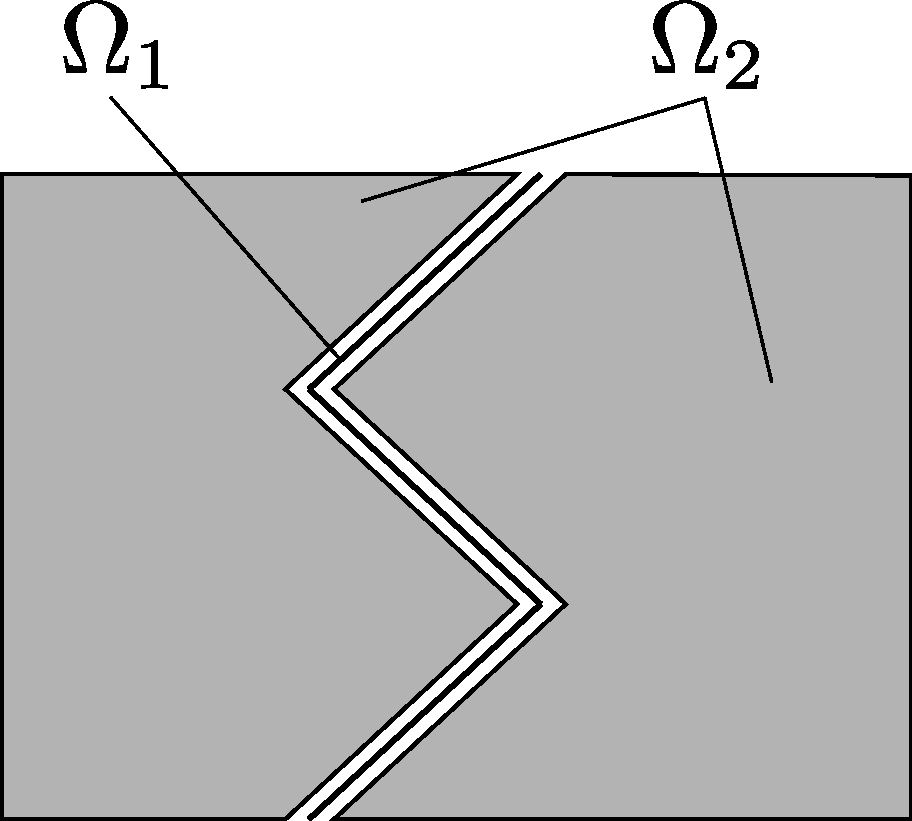
\includegraphics[width=0.25\textwidth]{figs/components} \hspace{25mm} 
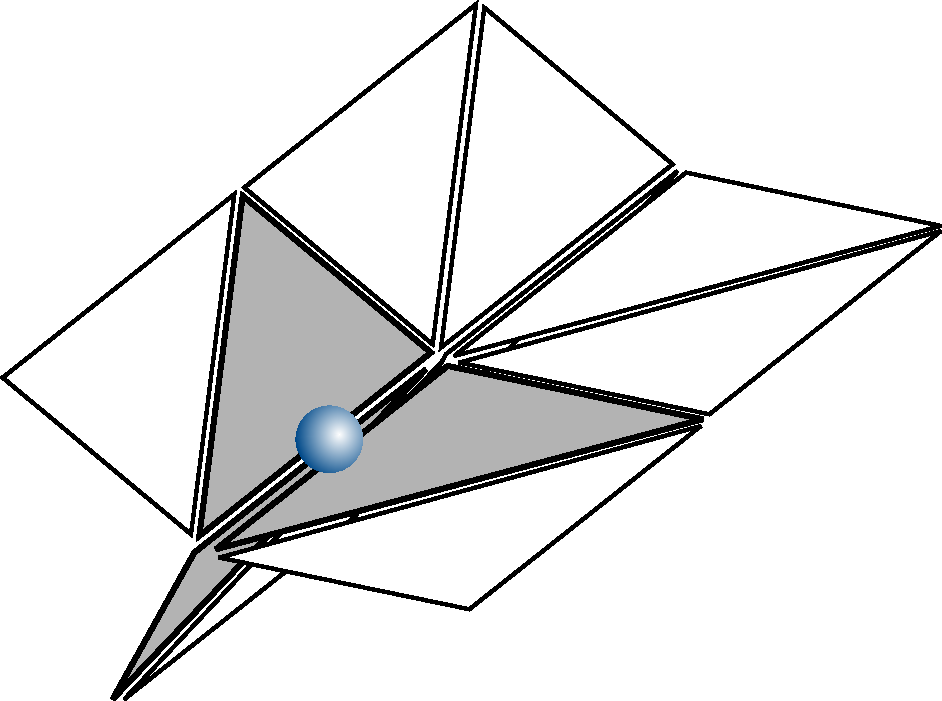
\includegraphics[width=0.30\textwidth]{figs/starlike-conf}
\end{center}
\caption{\label{fig:schemes}
Example of a two-dimensional problem: even single fracture gives rise to two components of the two-dimensional mesh (left);
example of three (shaded) triangles sharing a~single Lagrange multiplier in 3D (right).}
\end{figure}

\bibliographystyle{wileyj}
\bibliography{mh_theory}

\end{document}
